\documentclass{exam}
\usepackage{tikz}
\usepackage{subfig}
\usepackage{amsmath}
\usepackage[margin=1.0in]{geometry}
\pagestyle{empty}
\title{\textbf{Mock Test OMR Sheet}}
\begin{document}
\maketitle

\vspace{5mm}

\vspace{5mm}
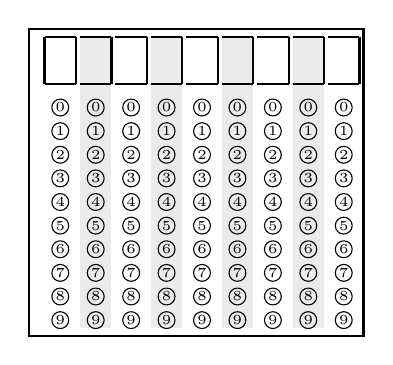
\begin{tikzpicture}[font=\small]
  % Define gradient colors
  \definecolor{lightblue}{RGB}{255,255,255}
  \definecolor{lightgray}{RGB}{235,235,235}

  % Create 9 columns for 9 digits
  \foreach \digit in {1,2,...,9} {
    % Determine background color (alternating)
    \pgfmathparse{mod(\digit,2)==1 ? 1 : 0}
    \ifnum\pgfmathresult=1
    \def\bgcolor{lightblue}
    \else
    \def\bgcolor{lightgray}
    \fi

    % Background rectangle for each column (tighter)
    \fill[\bgcolor] ({\digit * 0.45 - 0.2}, 0.5) rectangle ({\digit *
    0.45 + 0.2}, -3.2);

    % Hand-written digit box at the top of each column - only draw
    % left border for first box
    \ifnum\digit=1
    \draw[thick] ({\digit * 0.45 - 0.2}, 0.5) -- ({\digit * 0.45 - 0.2}, -0.1);
    \fi
    % Draw top, bottom, and right borders for all boxes
    \draw[thick] ({\digit * 0.45 - 0.2}, 0.5) -- ({\digit * 0.45 + 0.2}, 0.5);
    \draw[thick] ({\digit * 0.45 - 0.2}, -0.1) -- ({\digit * 0.45 + 0.2}, -0.1);
    \draw[thick] ({\digit * 0.45 + 0.2}, 0.5) -- ({\digit * 0.45 + 0.2}, -0.1);

    % Create rows for digits 0-9
    \foreach \number in {0,1,2,3,4,5,6,7,8,9} {
      \begin{scope}[yshift={-\number * 0.3 cm - 0.4 cm}]
        % Bubble for each digit position with number inside (tighter spacing)
        \node[draw, circle, inner sep=0.5pt, minimum size=6pt] at
        ({\digit * 0.45}, 0) {\tiny\number};
      \end{scope}
    }
  }

  % Draw border box around the entire OMR sheet (much tighter)
  \draw[thick] (0.05, 0.6) rectangle (4.3, -3.3);
\end{tikzpicture}
\end{document}
